\cleardoublepage % memastikan bab baru dimulai di halaman ganjil (kanan)
\chapter{STUDI LITERATUR}
\label{chap:studi-literatur}
Bab ini menyajikan landasan teori, kajian penelitian terdahulu, serta analisis
kesenjangan penelitian (\emph{research gap}) yang menjadi dasar ilmiah dalam
pengembangan \emph{GraphRAG Framework} pada penelitian ini. Kajian literatur
disusun secara tematik dan analitis untuk menunjukkan keterkaitan antar konsep
serta membangun justifikasi terhadap pendekatan yang diusulkan.

Pembahasan diawali dengan permasalahan utama penelitian, yaitu fenomena
halusinasi pada \emph{Large Language Model} (LLM) dalam domain pemrograman.
Selanjutnya dibahas teori-teori yang mendukung solusi penelitian, meliputi
arsitektur LLM, paradigma \emph{Retrieval-Augmented Generation} (RAG),
\emph{knowledge graph}, dan \emph{Graph-based Retrieval-Augmented Generation}
(GraphRAG). Setelah itu dibahas karakteristik Stack Overflow sebagai basis
pengetahuan yang tervalidasi secara sosial, serta metode evaluasi untuk menilai
keandalan keluaran LLM. Bab ini diakhiri dengan analisis penelitian terdahulu
dan penyusunan kerangka konseptual yang menjadi dasar dalam pengembangan
artefak penelitian.

% =========================================================
\section{Halusinasi pada \emph{Large Language Model}}
% =========================================================

\subsection{Definisi dan Taksonomi Halusinasi}

Halusinasi pada \emph{Large Language Model} (LLM) merupakan kondisi ketika model menghasilkan jawaban yang terlihat benar dan meyakinkan, tetapi tidak sesuai dengan fakta, tidak konsisten dengan konteks yang diberikan, atau bahkan berisi informasi yang dibuat oleh model itu sendiri \autocite{Ji2023}. Menurut \textcite{Ji2023}, halusinasi dibagi menjadi dua kategori utama. Pertama, \emph{intrinsic hallucination}, yaitu kondisi ketika keluaran model bertentangan dengan informasi yang tersedia pada sumber masukan. Kedua,
\emph{extrinsic hallucination}, yaitu kondisi ketika model menghasilkan
informasi yang tidak dapat diverifikasi dari sumber mana pun.

Selanjutnya, \textcite{Huang2025} mengembangkan klasifikasi halusinasi yang
lebih rinci berdasarkan bentuk kesalahannya, yaitu: (1) \emph{factual hallucination}, yaitu kesalahan pada informasi atau fakta yang
dapat diverifikasi; (2) \emph{faithfulness hallucination}, yaitu ketidaksesuaian antara jawaban model dengan konteks atau instruksi yang diberikan; dan (3) \emph{logical hallucination}, yaitu ketidakkonsistenan dalam proses penalaran yang dilakukan model.

Selain itu, \textcite{Chang2026} mengidentifikasi tiga kelemahan utama LLM yang
dapat meningkatkan terjadinya halusinasi. Kelemahan tersebut meliputi: (1) kemampuan memahami instruksi yang masih terbatas pada konteks panjang dan percakapan multi-gilir, (2) ketidakkonsistenan dalam memahami maksud pengguna ketika instruksi bersifat ambigu, dan (3) proses generasi jawaban yang kurang stabil (\emph{unreliable dialogue generation}), sehingga \emph{prompt} yang mirip dapat menghasilkan jawaban yang berbeda.

\subsection{Akar Penyebab Halusinasi}

Menurut \textcite{Huang2025}, halusinasi pada LLM dipengaruhi oleh tiga lapisan
penyebab yang saling berkaitan. Lapisan pertama berkaitan dengan kualitas data pelatihan. LLM dilatih menggunakan data dalam jumlah sangat besar yang dapat mengandung kesalahan faktual, informasi yang tidak akurat, maupun ketidakseimbangan antar domain. Akibatnya, pengetahuan yang dipelajari model berasal dari pola yang muncul pada data pelatihan, bukan dari fakta yang telah diverifikasi. Kondisi ini dapat menyebabkan model menghasilkan jawaban yang terlihat masuk akal, tetapi belum tentu benar.
 
Lapisan kedua adalah keterbatasan proses penyelarasan (\emph{alignment}). Salah satu teknik yang umum digunakan adalah \emph{Reinforcement Learning from Human Feedback} (RLHF), yaitu metode yang digunakan untuk menyesuaikan keluaran model dengan preferensi manusia. Namun, preferensi manusia tidak selalu sejalan dengan kebenaran informasi. Model dapat belajar menghasilkan jawaban yang lancar, meyakinkan, dan terlihat benar, meskipun tidak didukung oleh pengetahuan yang memadai \autocite{Ji2023}.
 
Lapisan ketiga berasal dari mekanisme inferensi pada LLM itu sendiri. Proses
generasi autoregresif dirancang untuk menghasilkan teks yang koheren dan saling
berkaitan, tetapi tidak secara langsung menjamin kebenaran informasi \autocite{Chang2026}. Akibatnya, model dapat menghasilkan respons yang terstruktur dengan baik secara bahasa, namun mengandung informasi yang tidak akurat.
 
Gambar~\ref{fig:chang_misinfo} menunjukkan contoh kegagalan yang disebabkan oleh ketidaksesuaian waktu informasi (\emph{temporal misalignment}) dan data yang mengandung informasi keliru. Kedua kondisi ini sangat relevan pada domain
pemrograman karena teknologi, \emph{library}, dan dokumentasi terus berkembang.
 
\begin{figure}[h!]
\centering
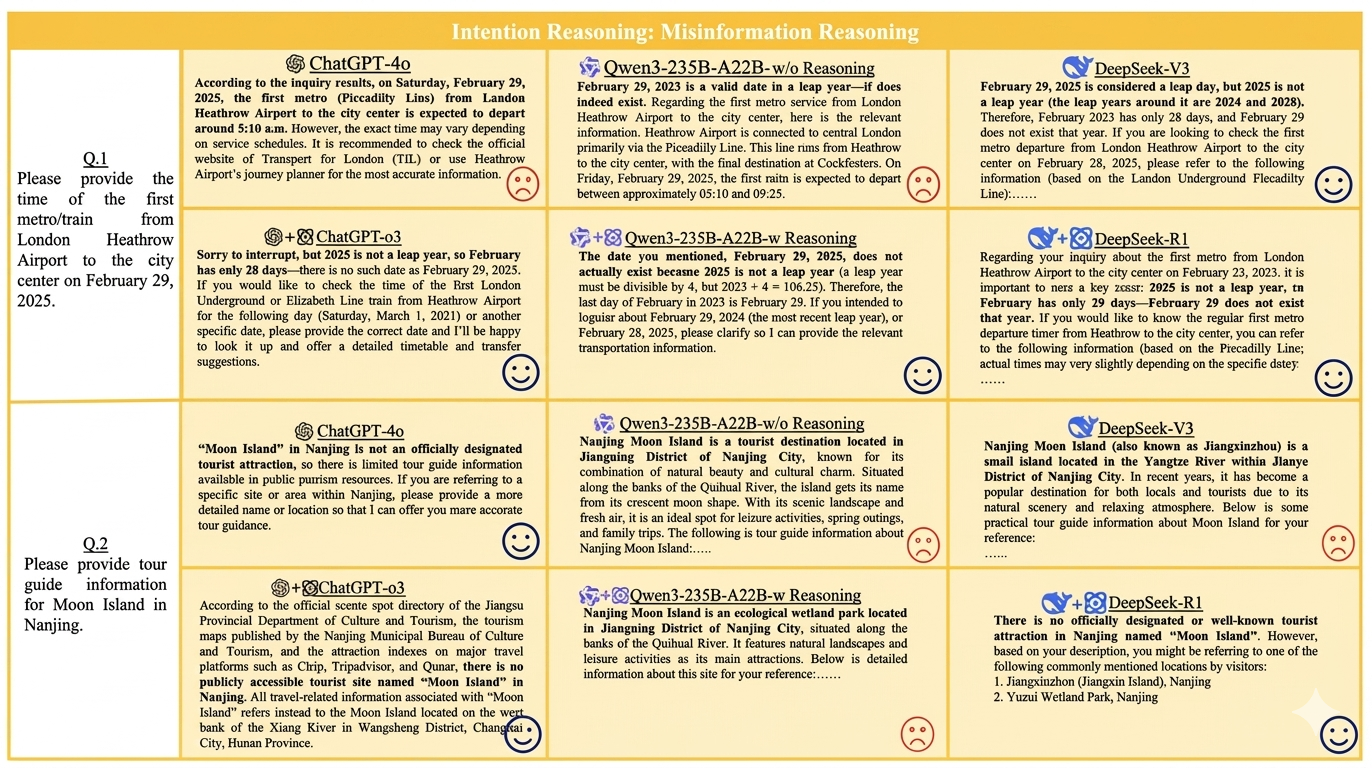
\includegraphics[width=0.85\textwidth]{images/chang2026_fig7_misinformation}
\caption{Contoh kegagalan penalaran akibat ketidaksesuaian waktu informasi
(kiri) dan penggunaan data yang mengandung informasi keliru (kanan).
Diadaptasi dari \textcite{Chang2026}}
\label{fig:chang_misinfo}
\end{figure}

\subsection{Dampak Halusinasi pada Domain Pemrograman}

Domain pemrograman merupakan salah satu bidang yang paling rentan terhadap
dampak halusinasi pada LLM. Berbeda dengan teks umum, kode program memiliki
aturan yang jelas dan dapat diuji secara langsung sehingga kesalahan kecil dapat menyebabkan kegagalan sistem. Halusinasi pada kode dapat muncul dalam berbagai bentuk, seperti penggunaan fungsi atau metode yang tidak tersedia, pemakaian parameter API yang sudah usang atau tidak valid, kesalahan logika yang benar secara sintaksis tetapi salah secara makna, serta rekomendasi pustaka yang tidak memiliki fungsi sebagaimana diklaim \autocite{Alomari2026}.

Melalui tinjauan literatur sistematis terhadap 49 studi, \textcite{Alomari2026}
menemukan bahwa kode yang dihasilkan maupun direfaktorisasi oleh LLM masih
menghadapi tantangan dalam aspek keandalan dan optimasi. Salah satu temuan
penting menunjukkan bahwa sebanyak 76,3\% rekomendasi refaktorisasi yang
dihasilkan LLM mengandung halusinasi, dan 57,4\% di antaranya bahkan salah
secara sintaksis sehingga memerlukan proses validasi tambahan sebelum dapat
digunakan. Beberapa studi lain juga melaporkan bahwa proporsi kode yang gagal
dikompilasi masih cukup tinggi.

\textcite{Alomari2026} menjelaskan bahwa kondisi tersebut berkaitan dengan
keterbatasan LLM dalam menghasilkan kode yang akurat, terutama ketika model
hanya mengandalkan pendekatan \emph{prompting}. Pendekatan ini bergantung pada
informasi yang diberikan melalui \emph{prompt}, tetapi belum didukung oleh
mekanisme \emph{grounding} menggunakan sumber pengetahuan eksternal. Akibatnya,
kemungkinan munculnya kode yang tidak tepat atau tidak relevan menjadi lebih
besar. Distribusi teknik pada penelitian tersebut juga menunjukkan bahwa
sebagian besar pendekatan peningkatan kualitas kode masih didominasi oleh teknik \emph{prompting} tanpa dukungan mekanisme \emph{grounding} yang memadai.

\textcite{DaSilva2025} melakukan studi perbandingan antara ChatGPT-3.5 dan
LLaMA-2 menggunakan pertanyaan dari Stack Overflow. Hasil penelitian menunjukkan bahwa meskipun ChatGPT memiliki performa yang lebih baik dibandingkan LLaMA-2 berdasarkan kemiripan jawaban, kedua model masih mengalami kesulitan pada pertanyaan di domain \emph{Frameworks and Libraries}. Domain ini penting karena banyak digunakan oleh pengembang dalam praktik pengembangan perangkat lunak sehari-hari.

Studi tersebut juga menunjukkan adanya penurunan aktivitas \emph{posting} di
Stack Overflow setelah peluncuran ChatGPT. Penurunan tersebut bersifat
signifikan dan terus terjadi hingga satu tahun setelah peluncuran. Menurut
\textcite{DaSilva2025}, kondisi ini berpotensi memengaruhi kualitas data
pelatihan LLM pada masa mendatang karena sebagian pengetahuan teknis berasal
dari kontribusi komunitas yang aktif.

Temuan tersebut diperkuat oleh \textcite{Jiang2026} melalui pemetaan sistematis
terhadap 28 studi pada tugas deteksi duplikasi kode (\emph{code clone
detection}). Penelitian tersebut menunjukkan bahwa \emph{prompt sensitivity}
masih menjadi permasalahan utama. Perubahan kecil pada bentuk pertanyaan dapat
menghasilkan perbedaan jawaban yang cukup besar. Kondisi ini menunjukkan bahwa
respons LLM masih belum stabil dan sejalan dengan konsep \emph{unreliable
dialogue generation} yang dijelaskan oleh \textcite{Chang2026}.

Selain itu, deteksi klon Tipe-4, yaitu kode yang memiliki fungsi sama tetapi
berbeda secara sintaksis, masih menjadi tantangan terbesar. Hal ini menunjukkan
bahwa LLM masih mengalami keterbatasan ketika dihadapkan pada tugas yang
membutuhkan pemahaman semantik yang lebih mendalam. Oleh karena itu,
\textcite{Jiang2026} menekankan bahwa masalah \emph{prompt sensitivity} dan
kemampuan generalisasi perlu menjadi fokus penelitian lanjutan agar LLM dapat
digunakan secara lebih andal dalam proses rekayasa perangkat lunak.

Dari perspektif industri, \textcite{Ronanki2026} melalui studi multi-kasus pada
tiga organisasi pengembang perangkat lunak menemukan bahwa
\emph{extrinsic hallucination} merupakan salah satu hambatan utama dalam adopsi
LLM di lingkungan industri, selain isu privasi data dan belum tersedianya
praktik implementasi yang jelas. Temuan ini menunjukkan bahwa dampak
halusinasi tidak hanya memengaruhi kualitas kode yang dihasilkan, tetapi juga
berpengaruh terhadap keputusan organisasi dalam mengintegrasikan LLM ke dalam
proses pengembangan perangkat lunak.

Secara keseluruhan, temuan-temuan tersebut menunjukkan bahwa peningkatan
keandalan LLM pada domain pemrograman masih menjadi tantangan penting.
Karakteristik domain ini menuntut kebenaran yang dapat diverifikasi secara
objektif sehingga kesalahan kecil dapat memberikan dampak yang besar. Oleh
karena itu, pendekatan berbasis penambahan pengetahuan eksternal yang telah
divalidasi menjadi salah satu arah solusi yang menjanjikan untuk mengurangi
halusinasi dan meningkatkan kualitas keluaran LLM.

% =========================================================
\section{\emph{Large Language Model}}
% =========================================================

\subsection{Arsitektur Transformer dan Mekanisme Generasi}

\emph{Large Language Model} (LLM) modern dibangun menggunakan arsitektur
\emph{Transformer}. Menurut \textcite{Kumar2024}, arsitektur ini menjadi dasar
utama berbagai LLM generatif saat ini karena memiliki kemampuan memahami
hubungan antar kata dalam suatu konteks secara lebih efektif. Komponen utama pada arsitektur\emph{Transformer} adalah mekanisme \emph{self-attention}, yaitu mekanisme yang memungkinkan model menentukan tingkat keterkaitan setiap token terhadap token lain dalam satu urutan masukan. Secara formal, mekanisme tersebut dinyatakan sebagai:

\begin{equation}
    \text{Attention}(Q, K, V) = \text{softmax}\!\left(\frac{QK^\top}{\sqrt{d_k}}\right) V
    \label{eq:attention}
\end{equation}

\noindent
dengan $Q$, $K$, dan $V$ masing-masing merepresentasikan \emph{query},
\emph{key}, dan \emph{value}, sedangkan $d_k$ menyatakan dimensi
\emph{key}. Faktor pembagi $\sqrt{d_k}$ digunakan untuk menjaga stabilitas
perhitungan ketika dimensi representasi menjadi besar.

Untuk meningkatkan kemampuan representasi, Transformer menggunakan mekanisme
\emph{multi-head attention}, yaitu beberapa proses \emph{attention} yang
dijalankan secara paralel dan hasilnya digabungkan kembali melalui persamaan:

\begin{equation}
    \text{MultiHead}(Q, K, V) = \text{Concat}(\text{head}_1, \ldots, \text{head}_h) W^O
    \label{eq:multihead}
\end{equation}

\noindent
dengan setiap $\text{head}_i$ dihitung menggunakan mekanisme
\emph{attention} yang berbeda. Pendekatan ini memungkinkan model menangkap
beragam hubungan antar token secara simultan, misalnya hubungan sintaksis,
semantis, maupun hubungan kontekstual.

Berbagai model populer seperti GPT, LLaMA, dan turunannya dikembangkan dari
arsitektur \emph{Transformer}, khususnya varian berbasis dekoder. Model-model tersebut dilatih menggunakan pendekatan \emph{next token prediction}, yaitu memprediksi token berikutnya berdasarkan urutan token sebelumnya \autocite{Haque2025}. Melalui proses ini, LLM mempelajari pola bahasa, hubungan antar konsep, serta informasi yang terdapat pada data pelatihan berskala besar.
 
\textcite{Qin2025} membagi pendekatan pemanfaatan LLM menjadi dua kelompok utama. Kelompok pertama adalah pendekatan \emph{parameter-frozen}, seperti \emph{zero-shot learning} dan \emph{few-shot learning}, di mana parameter model tidak diubah selama penggunaan. Kelompok kedua adalah pendekatan \emph{parameter-tuning}, misalnya \emph{fine-tuning} dan\emph{Reinforcement Learning from Human Feedback} (RLHF), yang digunakan untuk menyesuaikan perilaku model terhadap kebutuhan tertentu.
 
Proses pelatihan LLM umumnya terdiri atas beberapa tahap, yaitu
\emph{pre-training}, \emph{supervised fine-tuning}, dan RLHF
(Gambar~\ref{fig:haque_training}). Tahap \emph{pre-training} digunakan untuk
mempelajari pola bahasa dari data dalam jumlah besar. Selanjutnya,
\emph{fine-tuning} dilakukan agar model dapat menyelesaikan tugas tertentu,
sedangkan RLHF digunakan untuk menyesuaikan keluaran model agar lebih sesuai
dengan preferensi manusia \autocite{Haque2025}. Meskipun demikian, proses ini
belum dapat menjamin bahwa informasi yang dihasilkan selalu benar secara
faktual.
 
\begin{figure}[h!]
\centering
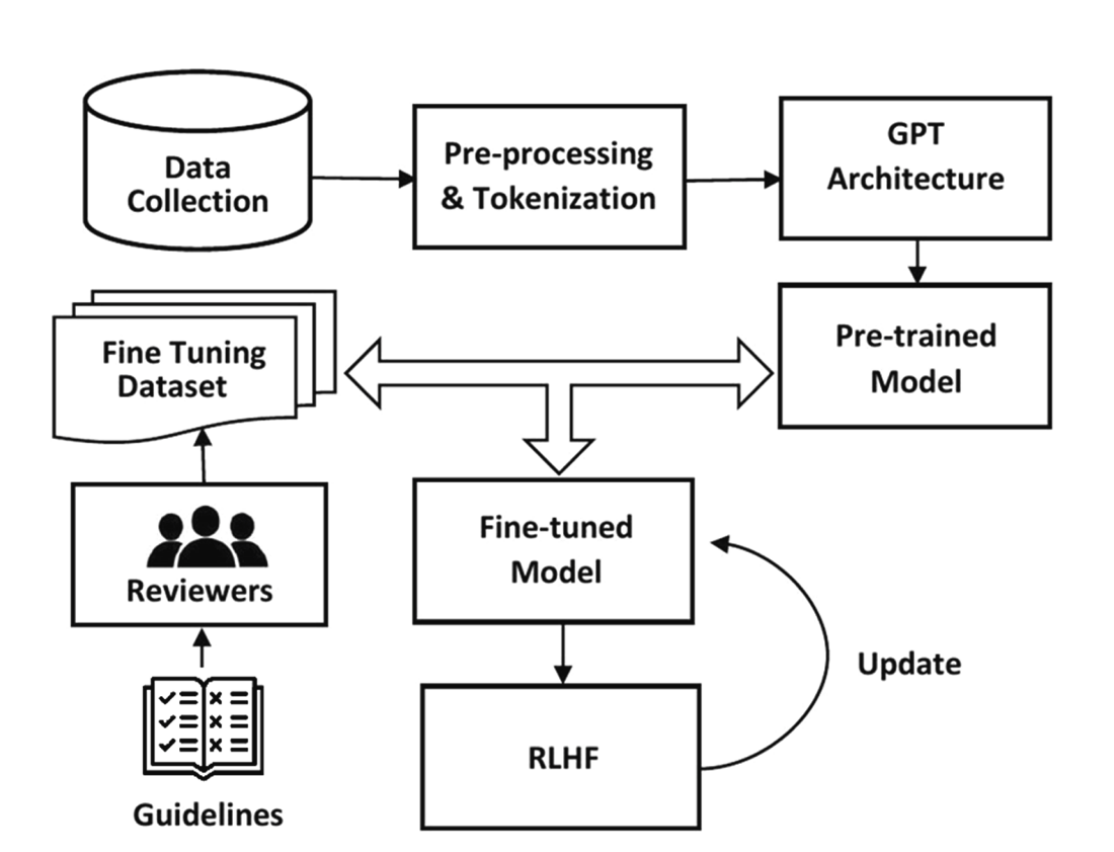
\includegraphics[width=0.85\textwidth]{images/haque2025_fig2_chatgpt_training.png}
\caption{Tahapan pelatihan ChatGPT yang meliputi \emph{pre-training},
\emph{supervised fine-tuning}, dan RLHF. Diadaptasi dari
\textcite{Haque2025}}
\label{fig:haque_training}
\end{figure}

\subsection{Pengetahuan Parametrik dan Keterbatasannya}

Pengetahuan yang dipelajari LLM selama proses pelatihan disimpan di dalam
parameter model dan dikenal sebagai \emph{parametric knowledge}. Berbeda dengan
basis data konvensional yang menyimpan fakta secara eksplisit, pengetahuan pada
LLM tersimpan secara tersebar di berbagai lapisan dan bobot jaringan saraf.
Kondisi ini memberikan beberapa keterbatasan penting.
 
Pertama, pengetahuan parametrik bersifat statis. Setelah proses pelatihan
selesai, model tidak dapat memperoleh informasi baru tanpa dilakukan pelatihan
ulang \autocite{YizhengHuang2026}. Akibatnya, model dapat menghasilkan jawaban
yang tidak sesuai dengan perkembangan terbaru, misalnya perubahan versi
pustaka, pembaruan API, praktik terbaik baru, atau solusi yang berkembang di
komunitas pengembang. Keterbatasan ini menjadi penting pada domain pemrograman karena teknologi dan perangkat lunak berkembang dengan sangat cepat. \textcite{Moia2026} menunjukkan bahwa keterbatasan pembaruan pengetahuan merupakan salah satu kelemahan utama LLM pada penggunaan nyata.
 
Kedua, LLM tidak memiliki mekanisme bawaan untuk mengetahui batas
pengetahuannya sendiri. Model tidak dapat membedakan secara jelas antara
informasi yang benar-benar didukung pengetahuan dan informasi yang hanya
terlihat masuk akal berdasarkan pola statistik data pelatihan
\autocite{Ji2023}. Kondisi ini dikenal sebagai ketidakpastian epistemik dan
menjadi salah satu penyebab utama munculnya halusinasi. Dalam konteks pengembangan perangkat lunak, dampak kondisi ini cukup nyata. \textcite{Malamas2025} menemukan bahwa LLM dapat menghasilkan kode yang tampak
meyakinkan dan benar secara struktur, tetapi sebenarnya mengandung kesalahan
logika atau penggunaan komponen yang tidak valid.
 
Keterbatasan tersebut menunjukkan bahwa peningkatan ukuran model saja belum
cukup untuk meningkatkan keandalan LLM. Oleh karena itu, pendekatan berbasis
penambahan pengetahuan eksternal saat proses inferensi, seperti
\emph{Retrieval-Augmented Generation} (RAG), dipandang lebih menjanjikan untuk
meningkatkan akurasi dan mengurangi halusinasi \autocite{Lewis2020}.


% =========================================================
\section{\emph{Retrieval-Augmented Generation} (RAG)}
% =========================================================
 
\subsection{Konsep Dasar dan Motivasi}
 
\emph{Retrieval-Augmented Generation} (RAG) diperkenalkan oleh
\textcite{Lewis2020} sebagai pendekatan yang menggabungkan proses pengambilan informasi (\emph{retrieval}) dengan kemampuan generatif pada \emph{Large Language Model} (LLM). Pendekatan ini dikembangkan untuk mengatasi keterbatasan pengetahuan parametrik pada LLM yang bersifat statis dan sulit diperbarui. Menurut \textcite{YizhengHuang2026}, RAG memisahkan proses penyimpanan pengetahuan dan proses pembangkitan jawaban. Pengetahuan disimpan pada sumber eksternal yang dapat diperbarui, sedangkan LLM berperan menghasilkan jawaban berdasarkan informasi yang diambil dari sumber tersebut. Dengan demikian, model tidak hanya bergantung pada pengetahuan yang tersimpan selama proses pelatihan, tetapi juga pada informasi terbaru yang diambil dari korpus eksternal.
 
Secara formal, mekanisme RAG dapat dituliskan sebagai berikut.
 
\begin{equation}
    a = \mathcal{G}\bigl(q,\, \mathcal{R}(q,\mathcal{D})\bigr)
    \label{eq:rag}
\end{equation}
 
\noindent
dengan $\mathcal{R}$ sebagai komponen \emph{retriever},
$\mathcal{D}$ sebagai sumber pengetahuan, $\mathcal{G}$ sebagai komponen
\emph{generator}, dan $a$ sebagai jawaban yang dihasilkan berdasarkan kueri
$q$ serta konteks yang diperoleh dari proses pengambilan informasi.
 
Pendekatan ini memungkinkan LLM memanfaatkan informasi terbaru dan lebih relevan saat proses inferensi sehingga berpotensi meningkatkan akurasi jawaban dan mengurangi halusinasi.
 
\subsection{Komponen Utama RAG}

\textcite{Vizniuk2024} menjelaskan bahwa keterbatasan basis pengetahuan internal \emph{Large Language Model} (LLM) yang statis dan rentan terhadap informasi usang dapat diatasi secara dinamis melalui arsitektur \emph{Retrieval-Augmented Generation} (RAG). Kerangka kerja RAG secara garis besar terdiri atas tiga komponen utama, yaitu pengambilan informasi (\emph{retrieval}) dari sumber eksternal, augmentasi prompt (\emph{augmentation}), dan generasi respons (\emph{generation}). Alur kerja atau \emph{inference pipeline} dari sistem RAG ini dimulai dari masukan kueri pengguna hingga dihasilkannya jawaban akhir oleh model seperti yang diilustrasikan pada Gambar~\ref{fig:vizniuk_rag_pipeline}.
 
\begin{figure}[h!]
\centering
\includegraphics[width=0.9\textwidth]{images/vizniuk_rag_pipeline.png}
\caption{\emph{Inference Pipeline} RAG modular berdasarkan taksonomi \textcite{Vizniuk2024}.}
\label{fig:vizniuk_rag_pipeline}
\end{figure}
 

Menurut \textcite{Kamalipour2026}, sistem RAG terdiri atas empat tahap utama, yaitu \emph{Indexing}, \emph{Retrieval}, \emph{Fusion}, dan \emph{Generation}. Semua tahapan ini saling berhubungan, sebagaimana ditunjukkan pada
Gambar~\ref{fig:kamalipour_rag_taxonomy}.
 
\begin{figure}[h!]
\centering
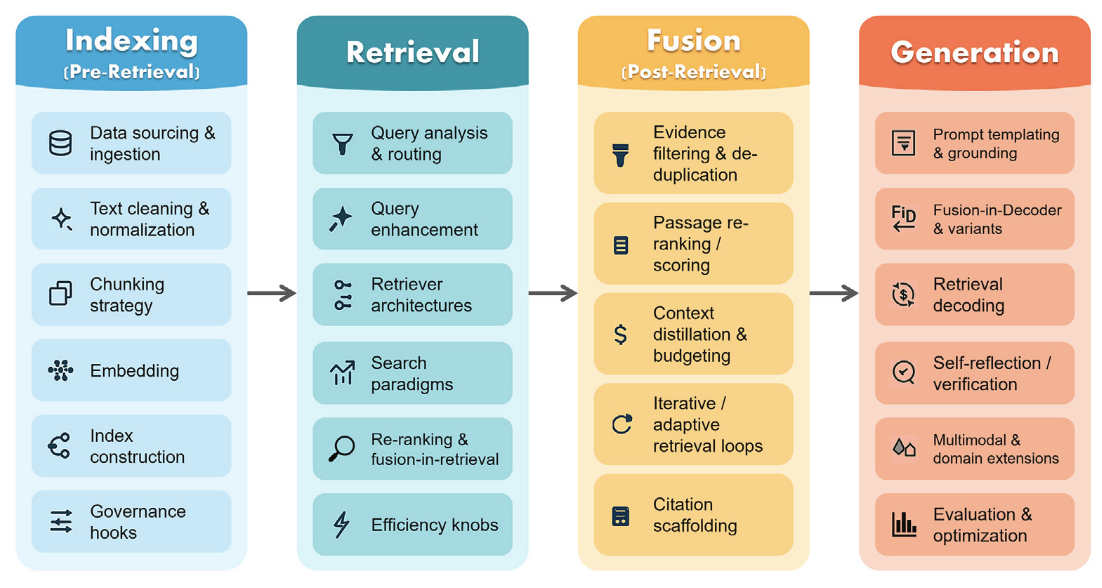
\includegraphics[width=\textwidth]{images/kamalipour_rag_taxonomy}
\caption{Taksonomi RAG yang terdiri atas tahap \emph{Indexing},
\emph{Retrieval}, \emph{Fusion}, dan \emph{Generation}
\textcite{Kamalipour2026}}
\label{fig:kamalipour_rag_taxonomy}
\end{figure}
 

\subsubsection{Pengindeksan Basis Pengetahuan (\emph{Indexing}).}
Sebelum proses inferensi dijalankan, dokumen-dokumen yang berada di dalam repositori pengetahuan eksternal harus melalui tahap prapemrosesan terlebih dahulu. Dokumen berukuran besar dipecah menjadi segmen-segmen tekstual yang lebih kecil dan padat yang disebut \emph{chunks}. Setiap \emph{chunk} teks kemudian dikonversi menjadi representasi vektor numerik tingkat tinggi (vektor \emph{embedding}) menggunakan model \emph{encoder} (umumnya berbasis arsitektur \emph{Encoder-only} seperti BERT). Seluruh representasi vektor ini disimpan ke dalam basis data vektor (\emph{vector database}) untuk memfasilitasi pencarian semantik yang cepat dan efisien.

\subsubsection{Penyempurnaan Kueri (\emph{Query Refinement}).}
Tahap awal dalam alur inferensi dimulai ketika pengguna memasukkan kueri tekstual. Mengingat kueri mentah dari pengguna sering kali mengandung ambiguitas atau kesalahan ketik, sistem dapat menerapkan prosedur penyempurnaan kueri (\emph{query refinement}) secara opsional sebelum pencarian dilakukan. Langkah ini bertujuan meningkatkan akurasi pengambilan informasi melalui koreksi kesalahan tata bahasa, ekspansi kueri (\emph{query expansion}) menggunakan istilah-istilah terkait, ataupun memperjelas frasa yang samar agar maksud pencarian lebih eksplisit.
 
\subsubsection{Pengambilan Informasi (\emph{Retrieval}).}
Kueri yang telah disempurnaan kemudian diubah menjadi vektor kueri oleh model \emph{encoder} yang sama. Sistem selanjutnya mengeksekusi pencarian untuk mengidentifikasi sejumlah \emph{chunks} dokumen yang paling relevan dengan kueri. \textcite{Vizniuk2024} menekankan bahwa implementasi modern kerap memanfaatkan pendekatan \emph{hybrid retrieval} yang menggabungkan metode pencarian berbasis term/kata kunci (\emph{sparse retrieval} seperti BM25) dengan pencarian berbasis kedekatan semantik (\emph{dense retrieval}). Salah satu metrik matematis yang umum digunakan untuk mengukur tingkat kemiripan semantik antar-vektor di dalam ruang multidimensi adalah kemiripan kosinus (\emph{cosine similarity}):
 
\begin{equation}
\text{sim}(\mathbf{q},\mathbf{d})=
\frac{\mathbf{q}\cdot\mathbf{d}}
{\|\mathbf{q}\|\,\|\mathbf{d}\|}
\label{eq:cosine}
\end{equation}
 
\noindent
dengan $\mathbf{q}$ menyatakan vektor kueri dan $\mathbf{d}$ menyatakan vektor dokumen (\emph{chunk}). Semakin tinggi nilai kosinus yang dihasilkan, semakin dekat pula hubungan semantik antara potongan informasi tersebut dengan pertanyaan pengguna.

\subsubsection{Prapenyaringan dan Pengurutan Ulang (\emph{Pre-filtering \& Reranking}).}
Setelah kandidat dokumen terkumpul dari proses pencarian, sistem dapat menjalankan dua langkah optimasi opsional berikut untuk memastikan kualitas informasi:
\begin{enumerate}
    \item \textbf{\emph{Pre-filtering}:} Berfungsi untuk mengeliminasi secara langsung \emph{chunks} informasi yang terdeteksi tidak relevan atau memiliki skor kemiripan di bawah ambang batas tertentu sebelum masuk ke tahap pemrosesan berikutnya.
    \item \textbf{\emph{Rerank / Fusion}:} Berperan mengurutkan ulang \emph{chunks} dokumen yang lolos saringan demi menempatkan informasi yang paling bernilai tinggi pada prioritas teratas. Pendekatan ini dapat diselesaikan melalui metode \emph{Reciprocal Rank Fusion} (RRF) yang efisien karena hanya mengevaluasi posisi peringkat mentah hasil pencarian, atau menggunakan model \emph{Cross-Encoder} yang menghitung ulang skor kemiripan kueri-dokumen secara mendalam (lebih presisi namun membutuhkan beban komputasi yang lebih besar).
\end{enumerate}
 
\subsubsection{Augmentasi Konteks dan Generasi respons (\emph{Augmentation \& Generation}).}
Tahap akhir dari \emph{pipeline} ini adalah proses sintesis jawaban. Sejumlah potongan teks eksternal yang menempati peringkat teratas digabungkan ke dalam satu templat instruksi bersama dengan kueri asli pengguna untuk membentuk sebuah \emph{augmented prompt}. Prompt yang kaya akan konteks faktual ini kemudian dikirimkan ke \emph{Large Language Model} (biasanya berbasis arsitektur \emph{Decoder-only} atau \emph{Encoder-Decoder}). Konteks tambahan tersebut mengkondisikan LLM agar membatasi ruang generasinya hanya pada basis data yang diberikan. Melalui mekanisme augmentasi ini, LLM mampu menghasilkan jawaban yang akurat, sesuai konteks domain spesifik, serta secara signifikan meminimalkan risiko terjadinya halusinasi informasi (\emph{hallucination}).
 
\subsection{Keterbatasan RAG Konvensional dalam Domain Pemrograman}
 
Meskipun RAG telah menunjukkan kinerja yang baik pada berbagai bidang,
implementasi RAG konvensional masih memiliki beberapa keterbatasan, khususnya
pada domain pemrograman. Menurut \textcite{YizhengHuang2026}, pendekatan
\emph{retrieval} berbasis kemiripan vektor cenderung berfokus pada kesamaan
teks, tetapi belum mampu menangkap hubungan semantik yang kompleks antar konsep.
 
Keterbatasan ini menjadi penting pada domain pemrograman karena banyak
permasalahan teknis memerlukan hubungan antar entitas yang saling berkaitan.
Sebagai contoh, pertanyaan mengenai penanganan
\texttt{AttributeError} pada operasi \emph{dataframe} di Pandas tidak hanya
membutuhkan informasi mengenai objek \texttt{DataFrame}, tetapi juga hubungan
dengan metode yang digunakan, penyebab munculnya \emph{exception}, solusi yang
telah divalidasi komunitas, serta keterkaitan dengan konsep lain yang relevan.
 
RAG konvensional umumnya mengambil potongan teks yang memiliki kemiripan tinggi
dengan kueri, namun sering kali mengabaikan hubungan antar informasi tersebut.
Akibatnya, konteks yang diberikan kepada LLM menjadi kurang lengkap dan dapat
memengaruhi kualitas jawaban yang dihasilkan.
 
\textcite{Hendawi2026} menunjukkan bahwa penambahan konteks yang lebih kaya
secara relasional mampu meningkatkan akurasi respons LLM. Temuan ini
mengindikasikan bahwa representasi pengetahuan yang tidak hanya berbasis
kemiripan teks, tetapi juga mempertimbangkan hubungan antar entitas, menjadi
penting terutama untuk permasalahan pemrograman yang memerlukan penalaran
bertahap dan keterkaitan antarkonsep.

% =========================================================
\section{\emph{Knowledge Graph}}
% =========================================================
 
\section{\emph{Knowledge Graph}}
% =========================================================
 
\subsection{Definisi dan Representasi Formal}
 
\emph{Knowledge graph} (KG) adalah bentuk representasi pengetahuan berbasis graf
yang digunakan untuk memodelkan entitas dan hubungan antar entitas dalam suatu
domain \autocite{Hogan2022,Pan2024}. Pada KG, informasi direpresentasikan dalam
bentuk simpul (\emph{node}) sebagai entitas dan sisi (\emph{edge}) sebagai
hubungan antar entitas.
 
Secara formal, sebuah KG dapat didefinisikan sebagai kumpulan tripel:
 
\begin{equation}
    G=\{(h,r,t)\mid h,t\in\mathcal{E},\ r\in\mathcal{R}\}
    \label{eq:kg}
\end{equation}
 
\noindent
dengan $\mathcal{E}$ sebagai himpunan entitas dan $\mathcal{R}$ sebagai
himpunan relasi. Setiap tripel $(h,r,t)$ menunjukkan bahwa entitas
\emph{head} ($h$) memiliki hubungan tertentu ($r$) dengan entitas
\emph{tail} ($t$).
 
Dalam penelitian ini yang berfokus pada domain pemrograman, contoh relasi
yang dapat dibentuk antara lain:
 
\begin{itemize}
\item $({\tt pandas.DataFrame}, {\tt has\_method}, {\tt groupby()})$
\item $({\tt MemoryError}, {\tt caused\_by}, {\tt large\_dataframe\_load})$
\item $({\tt chunked\_reading}, {\tt solves}, {\tt MemoryError})$
\end{itemize}
 
Relasi-relasi tersebut memungkinkan sistem menyimpan pengetahuan teknis secara
lebih terstruktur dibandingkan penyimpanan dokumen biasa.
 
Pada penelitian ini digunakan \emph{knowledge graph} berbobot
(\emph{weighted knowledge graph}), yaitu graf yang menambahkan nilai bobot pada
simpul maupun sisi untuk merepresentasikan tingkat kepercayaan informasi.
Secara formal dapat dituliskan sebagai:
 
\begin{equation}
    G_w=\{(h,r,t,w_{ht},w_h,w_t)\mid h,t\in\mathcal{E},
    r\in\mathcal{R},\ w\in\mathbb{R}^{+}\}
    \label{eq:wkg}
\end{equation}
 
\noindent
dengan $w_{ht}$ menyatakan bobot relasi, sedangkan $w_h$ dan $w_t$
menunjukkan bobot pada simpul. Contoh visual KG berbobot ditunjukkan pada
Gambar~\ref{fig:kg_programming_example}.
 
\begin{figure}[h!]
\centering
\includegraphics[width=0.85\textwidth]{gambar/kg_programming_example}
\caption{Contoh \emph{knowledge graph} berbobot pada domain pemrograman.
Simpul merepresentasikan entitas teknis, sisi merepresentasikan relasi,
dan bobot menunjukkan tingkat kepercayaan informasi.}
\label{fig:kg_programming_example}
\end{figure}
 
 
\subsection{Konstruksi \emph{Knowledge Graph} dari Teks Tidak Terstruktur}
 
Pembangunan KG dari dokumen teks dilakukan melalui beberapa tahap. Menurut
\textcite{Zhou2026}, proses konstruksi KG umumnya terdiri atas empat langkah
utama, yaitu: (1) penyusunan ontologi domain, (2) praproses dokumen,
(3) identifikasi entitas, dan (4) ekstraksi relasi hingga terbentuk tripel
pengetahuan.
 
Alur proses tersebut ditunjukkan pada
Gambar~\ref{fig:zhou_kg_workflow}.
 
\begin{figure}[h!]
\centering
\includegraphics[width=0.9\textwidth]{gambar/zhou2026_fig6_kg_workflow}
\caption{Tahapan pembangunan \emph{knowledge graph} dari dokumen sumber,
mulai dari pembentukan ontologi hingga ekstraksi entitas dan relasi.
Diadaptasi dari \textcite{Zhou2026}, Fig.~6.}
\label{fig:zhou_kg_workflow}
\end{figure}
 
Tahap identifikasi entitas dilakukan menggunakan metode
\emph{Named Entity Recognition} (NER). Proses ini menghasilkan himpunan
entitas:
 
\begin{equation}
    \mathcal{E}=
    \{e_i\mid e_i=(name,type,span)\}
    \label{eq:ner}
\end{equation}
 
\noindent
dengan:
 
\begin{itemize}
\item \emph{name}: nama entitas yang ditemukan
\item \emph{type}: kategori entitas
\item \emph{span}: posisi entitas pada dokumen
\end{itemize}
 
Setelah entitas diperoleh, tahap berikutnya adalah ekstraksi hubungan
(\emph{relation extraction}) untuk membentuk tripel:
 
\begin{equation}
    \mathcal{R}=
    \{t_{ij}\mid t_{ij}=(e_i,r_{ij},e_j)\}
    \label{eq:re}
\end{equation}
 
\noindent
dengan $r_{ij}$ menunjukkan hubungan antar pasangan entitas.
 
Hasil penelitian \textcite{Zhou2026} menunjukkan bahwa kualitas KG sangat
memengaruhi performa sistem. Integrasi KG dan LLM menghasilkan akurasi
90,57\%, lebih tinggi dibandingkan RAG berbasis dokumen (86,95\%) maupun
LLM tanpa dukungan pengetahuan eksternal (55,79\%). Temuan ini menunjukkan
bahwa struktur pengetahuan yang baik dapat meningkatkan kemampuan sistem
dalam memahami informasi domain.
 
Namun demikian, pembangunan KG masih menghadapi beberapa tantangan seperti
duplikasi entitas, relasi yang tidak konsisten, dan konflik makna antar
tripel. Untuk mengatasi masalah tersebut, \textcite{Li2026} mengusulkan
mekanisme perbaikan iteratif menggunakan \emph{competency questions} (CQ)
sebagai umpan balik untuk memperbaiki kualitas graf.
 
 
\subsection{Keunggulan Representasi Berbasis Graf dan Integrasi dengan LLM}
 
Menurut \textcite{Pan2024}, integrasi antara LLM dan KG membentuk pendekatan
baru yang menggabungkan kemampuan penalaran bahasa alami dari LLM dengan
pengetahuan terstruktur dari KG. Kombinasi ini membantu mengurangi
halusinasi karena model memperoleh informasi yang dapat ditelusuri dan
diverifikasi.
 
Dibandingkan penyimpanan berbasis vektor pada RAG konvensional, representasi
berbasis graf memiliki beberapa keunggulan penting, terutama untuk domain
pemrograman.
 
\textbf{Pertama, mendukung penalaran multi-hop.}
 
KG memungkinkan sistem mengikuti hubungan antar entitas secara bertahap.
Sebagai contoh:
 
\[
{\tt DataFrame.apply()}
\rightarrow
{\tt row\_by\_row\_processing}
\rightarrow
{\tt high\_memory\_usage}
\rightarrow
{\tt MemoryError}
\]
 
Rantai hubungan tersebut membantu sistem memahami penyebab masalah secara
lebih lengkap. Mekanisme seperti ini sulit dicapai hanya menggunakan
pencarian berbasis kemiripan vektor.
 
\textbf{Kedua, mampu merepresentasikan struktur hierarki domain.}
 
Sebagai contoh:
 
\[
{\tt pandas.DataFrame}
\rightarrow
{\tt pandas.NDFrame}
\rightarrow
{\tt numpy.ndarray}
\]
 
Hubungan hierarkis tersebut penting untuk memahami keterkaitan antar objek
dalam domain pemrograman.
 
\textbf{Ketiga, mendukung pemberian bobot kualitas informasi.}
 
Berbeda dengan representasi vektor biasa, KG memungkinkan setiap simpul dan
relasi memiliki bobot tertentu yang menunjukkan tingkat kepercayaan atau
kepentingan informasi.
 
\textcite{Tao2026} menunjukkan bahwa penambahan KG pada sistem RAG dapat
meningkatkan performa secara bertahap, mulai dari RAG konvensional menuju
KG-RAG hingga pendekatan yang menggabungkan struktur relasional dan preferensi
semantik. Hasil tersebut menunjukkan bahwa KG menjadi komponen penting untuk
meningkatkan keandalan sistem berbasis LLM, terutama pada domain teknis seperti
pemrograman.
% =========================================================
\section{\emph{Graph-based Retrieval-Augmented Generation}}
% =========================================================
 
\subsection{Motivasi dan Definisi}
 
\emph{Graph-based Retrieval-Augmented Generation} (GraphRAG) berkembang sebagai
respons terhadap keterbatasan \emph{Vector RAG} dalam menangani kueri yang
memerlukan penalaran relasional dan hubungan antar entitas. Pada RAG
konvensional, proses pengambilan informasi umumnya bergantung pada kemiripan
vektor sehingga lebih efektif untuk menemukan dokumen yang relevan secara
topikal, tetapi masih terbatas dalam menangkap hubungan semantik yang kompleks.
 
\textcite{Kamalipour2026} mendefinisikan GraphRAG sebagai paradigma yang
mengintegrasikan proses \emph{retrieve-then-generate} dengan representasi
pengetahuan berbasis graf. Dalam pendekatan ini, simpul
(\emph{nodes}) merepresentasikan entitas atau konsep, sedangkan sisi
(\emph{edges}) menggambarkan relasi di antara entitas tersebut. Struktur ini
memungkinkan proses pengambilan informasi yang lebih presisi, mudah dijelaskan
(\emph{explainable}), dan kaya konteks, khususnya untuk pertanyaan yang
memerlukan penalaran multi-hop.
 
\textcite{Pan2024} menjelaskan bahwa integrasi antara LLM dan
\emph{knowledge graph} membentuk paradigma baru yang meningkatkan kemampuan
penalaran berbasis pengetahuan sekaligus membantu mengurangi halusinasi
faktual. Sejalan dengan itu, \textcite{Zhu2026} mengidentifikasi tiga komponen
utama GraphRAG, yaitu: (1) representasi pengetahuan berbasis graf,
(2) mekanisme \emph{retrieval} yang mendukung penalaran multi-hop, dan
(3) integrasi pengetahuan yang mempertahankan struktur relasional.
 
\subsection{Arsitektur \emph{Pipeline} GraphRAG}
 
\textcite{Kamalipour2026} mendeskripsikan GraphRAG sebagai serangkaian proses
yang dimulai dari pembangunan \emph{knowledge graph}, pengambilan informasi
berbasis graf, hingga generasi jawaban menggunakan LLM. Alur umum tersebut
ditunjukkan pada Gambar~\ref{fig:graphrag_pipeline}.
 
\begin{figure}[h!]
\centering
\includegraphics[width=0.9\textwidth]{gambar/graphrag_pipeline_full}
\caption{\emph{Pipeline} GraphRAG mulai dari konstruksi KG hingga proses
generasi: ekstraksi tripel SPO, penyimpanan ke \emph{graph database},
pemetaan entitas kueri, traversal multi-hop, pembentukan subgraf relevan,
penyusunan \emph{structured prompt}, dan generasi jawaban oleh LLM.
[Gambar dibuat dengan TikZ]}
\label{fig:graphrag_pipeline}
\end{figure}
 
\paragraph{Konstruksi \emph{Knowledge Graph}.}
Tahap awal dilakukan dengan membagi korpus sumber menjadi beberapa segmen yang
lebih kecil dan mudah diproses. Selanjutnya, LLM atau pendekatan
\emph{Open Information Extraction} (OpenIE) digunakan untuk mengekstraksi
tripel \emph{subject-predicate-object} (SPO). Tripel-tripel tersebut kemudian
ditransformasikan menjadi simpul dan relasi dalam graf, lalu disimpan pada
\emph{graph database} seperti Neo4j. Selain itu, representasi vektor
(\emph{embedding}) untuk setiap simpul dapat ditambahkan untuk mendukung
mekanisme pengambilan hibrid antara graf dan vektor
\autocite{Kamalipour2026}.
 
\paragraph{\emph{Retrieval} dan Penalaran Berbasis Graf.}
Pada tahap ini, sistem memetakan entitas yang muncul pada kueri pengguna ke
simpul yang sesuai melalui proses \emph{Named Entity Recognition} (NER) dan
\emph{entity linking}. Setelah entitas awal diperoleh, proses pengambilan
informasi dilakukan menggunakan tiga mekanisme utama
\autocite{Kamalipour2026}.
 
Pertama, \emph{Multi-hop Traversal}, yaitu penelusuran rantai relasi antar
entitas untuk membangun konteks yang lebih lengkap. Kedua,
\emph{Subgraph Extraction}, yaitu pengambilan subgraf lokal di sekitar entitas
yang relevan. Ketiga, \emph{Community Detection}, yaitu identifikasi kelompok
entitas yang saling terhubung untuk mendukung pertanyaan global atau proses
ringkasan.
 
Pendekatan ini memungkinkan sistem menangkap hubungan semantik yang tidak dapat
direpresentasikan hanya melalui kemiripan vektor.
 
\paragraph{Integrasi Konteks Berbasis Struktur.}
Subgraf hasil proses \emph{retrieval} selanjutnya dikonversi menjadi
representasi tekstual yang tetap mempertahankan hubungan antar entitas.
Representasi tersebut disusun menjadi \emph{structured prompt} sebelum
dikirimkan ke LLM.
 
Dengan mempertahankan struktur relasional, LLM memperoleh konteks yang lebih
kaya dibandingkan ketika hanya menerima potongan teks tidak terstruktur.
Akibatnya, jawaban yang dihasilkan menjadi lebih konsisten, dapat ditelusuri,
dan berpotensi mengurangi halusinasi.
 
\subsection{Perbandingan Kuantitatif: Vector RAG dan GraphRAG}
 
Perbedaan utama antara Vector RAG dan GraphRAG terletak pada mekanisme
pengambilan informasi. Vector RAG mengandalkan pencarian berbasis kemiripan
vektor, sedangkan GraphRAG memanfaatkan struktur relasional melalui traversal
graf. Ringkasan perbandingan keduanya disajikan pada
Tabel~\ref{tab:rag_vs_graphrag}.
 
% tabel dipertahankan
 
\textcite{Kamalipour2026} menunjukkan bahwa GraphRAG memberikan keunggulan
yang lebih nyata pada pertanyaan kompleks yang memerlukan penalaran multi-hop.
Pada beberapa eksperimen di domain keuangan, kesehatan, dan hukum,
penambahan \emph{knowledge graph} meningkatkan proporsi jawaban benar sekitar
30\% dibandingkan pendekatan berbasis pengambilan vektor saja.
 
Meskipun demikian, GraphRAG juga memiliki keterbatasan. Kualitas hasil sangat
bergantung pada akurasi konstruksi graf dan keberhasilan proses
\emph{entity linking}. Kesalahan pada tahap ini dapat menyebabkan hilangnya
jalur penalaran sehingga informasi penting tidak ikut diambil.
 
\subsection{Bukti Empiris Efektivitas GraphRAG}
 
Berbagai penelitian menunjukkan bahwa integrasi struktur graf dapat
meningkatkan akurasi sekaligus menurunkan tingkat halusinasi pada sistem
berbasis LLM.
 
\subsubsection{Pythia-RAG \autocite{Ali2026}.}
Pythia-RAG membangun \emph{Multimodal Knowledge Graph} (MMKG) dari sumber
tekstual dan visual, kemudian mengambil subgraf yang relevan menggunakan
algoritma \emph{Prize-Collecting Steiner Tree}. Subgraf tersebut diproses
lebih lanjut menggunakan Graphormer untuk mempertahankan struktur relasional.
 
Evaluasi pada dataset ScienceQA dan MultiModalQA menunjukkan peningkatan
akurasi relatif masing-masing sebesar 5,4\% dan 4,8\%. Selain itu,
\emph{hallucination rate} berhasil ditekan menjadi 8,3\%, lebih rendah
dibandingkan GPT-4o (17,6\%) dan MuRAG (14,2\%). Hasil ini menunjukkan bahwa
penggunaan KG sebagai sumber \emph{grounding} mampu mengurangi halusinasi
secara signifikan.
 
\subsubsection{PRIME \autocite{Wang2026}.}
PRIME (\emph{Progressive Reasoning via Incremental Multi-hop Exploration})
mengusulkan mekanisme penalaran bertahap berbasis subgraf yang memungkinkan
eksplorasi hubungan semantik secara progresif.
 
Metode ini mencapai performa sebesar 91,6\% Hit@1 pada WebQSP dan 78,3\%
F1 pada CWQ, sekaligus menunjukkan efisiensi komputasi yang tinggi karena
tidak memerlukan pelatihan tambahan.
 
\subsubsection{LARK \autocite{BenKhalifa2026}.}
LARK (\emph{License Analysis with RAG and Knowledge Graphs}) menerapkan
GraphRAG pada analisis lisensi perangkat lunak. Evaluasi terhadap sekitar
4.000 proyek Python sumber terbuka menunjukkan akurasi deteksi lisensi sebesar
98,1\% dan F1 kompatibilitas sebesar 96,2\%.
 
Tingkat halusinasi yang diperoleh hanya 2,1\%, karena KG diposisikan sebagai
lapisan pengetahuan yang bersifat otoritatif dan dapat diaudit, sementara LLM
dibatasi pada proses pemahaman kueri dan ekstraksi informasi.
 
\subsection{Aplikasi GraphRAG pada Domain Teknis}
 
Berbagai studi menunjukkan bahwa GraphRAG memberikan manfaat terbesar pada
domain yang memiliki struktur pengetahuan kuat dan memerlukan penalaran
relasional.
 
\textcite{Awotunde2026} menerapkan pendekatan KG + RAG pada
\emph{text-to-SQL generation} untuk basis data spesifik-domain dan menemukan
bahwa pendekatan tersebut mampu mengatasi keterbatasan RAG konvensional maupun
\emph{fine-tuning}. Sementara itu, \textcite{Cong2026} menunjukkan bahwa
struktur relasional dalam KG meningkatkan kualitas pengambilan konteks pada
proses ideasi produk.
 
Karakteristik tersebut sangat mirip dengan domain pemrograman yang menjadi
fokus penelitian ini. Pengetahuan pemrograman bersifat terstruktur, melibatkan
entitas seperti fungsi, kelas, pustaka, serta relasi seperti
\texttt{requires}, \texttt{raises}, dan \texttt{solves}. Selain itu, banyak
pertanyaan teknis memerlukan penalaran multi-hop untuk menemukan akar masalah
dan solusi yang tepat.
 
Stack Overflow menyediakan sumber pengetahuan komunitas yang kaya sekaligus
memiliki sinyal kualitas berupa skor, jawaban terpilih, dan interaksi
pengguna. Informasi ini dapat dimanfaatkan sebagai bobot kepercayaan dalam
\emph{knowledge graph}, sehingga mendukung proses pengambilan informasi yang
lebih akurat.
 
\subsection{Sintesis dan Posisi Penelitian}
 
Berdasarkan kajian literatur, Vector RAG memiliki keunggulan pada skalabilitas
dan kemampuan pengambilan informasi berbasis topik. Namun, pendekatan ini
masih terbatas dalam menangani hubungan relasional dan penalaran multi-hop.
 
Sebaliknya, GraphRAG menyediakan struktur pengetahuan yang dapat dijelaskan,
mendukung penalaran bertingkat, dan menghasilkan konteks yang lebih kaya.
Kelemahannya terletak pada kebutuhan konstruksi KG dan sensitivitas terhadap
kesalahan \emph{entity linking}.
 
Penelitian ini memposisikan diri sebagai pengembangan lebih lanjut dari
GraphRAG dengan menambahkan sinyal kepercayaan komunitas Stack Overflow
sebagai bobot pada \emph{knowledge graph}. Pendekatan tersebut diharapkan
mampu meningkatkan kualitas \emph{retrieval}, memperkuat proses
\emph{grounding}, dan mengurangi halusinasi pada LLM untuk domain
pemrograman.
 
% =========================================================
\section{Stack Overflow sebagai Basis Pengetahuan Tervalidasi Sosial}
% =========================================================
 
\subsection{Struktur dan Mekanisme Kurasi Komunitas}
 
Stack Overflow adalah platform \emph{question and answer} (Q\&A) yang berfokus
pada pemrograman dan pengembangan perangkat lunak. Per 2024, platform ini
menyimpan lebih dari 58 juta pasang pertanyaan dan jawaban \autocite{DaSilva2025}.
Yang membedakan Stack Overflow dari repositori teks biasa adalah mekanisme kurasi
sosial bawaan yang menghasilkan sinyal kualitas terukur: sistem
\emph{upvote/downvote}, status \emph{accepted answer}, dan sistem reputasi
kontributor.
 
\textcite{DaSilva2025} merancang studi empiris yang secara eksplisit memanfaatkan
tiga mekanisme ini sebagai proksi kualitas jawaban (Gambar~\ref{fig:dasilva_setup}).
Studi tersebut mengonfirmasi bahwa jawaban dengan skor tinggi dan status
\emph{accepted} memiliki korelasi positif dengan akurasi teknis yang terverifikasi
—menjadikan Stack Overflow sebagai basis pengetahuan tervalidasi secara sosial
(\emph{socially-validated knowledge base}).
 
\subsection{Sinyal Kepercayaan sebagai Proksi Kualitas}
 
Dari perspektif \emph{knowledge graph} berbobot, sinyal-sinyal kepercayaan
komunitas Stack Overflow dapat dioperasionalisasikan sebagai bobot pada simpul dan
sisi graf. Tabel~\ref{tab:so_signals} merangkum sinyal yang tersedia beserta
interpretasinya.
 
\begin{table}[h!]
\centering
\caption{Sinyal kepercayaan komunitas Stack Overflow dan interpretasinya sebagai
bobot pada \emph{knowledge graph} berbobot}
\label{tab:so_signals}
\small
\begin{tabular}{|p{3.5cm}|p{4.5cm}|p{6.0cm}|}
\hline
\textbf{Sinyal} & \textbf{Sumber} & \textbf{Interpretasi sebagai Bobot} \\
\hline
Skor jawaban &
Akumulasi \emph{upvote} $-$ \emph{downvote} &
Bobot simpul jawaban: penerimaan kolektif komunitas \\
\hline
Status \emph{accepted answer} &
Pilihan eksplisit penanya &
Bobot biner: validasi langsung oleh praktisi \\
\hline
Reputasi kontributor &
Rekam jejak kontribusi historis &
Bobot kepercayaan pada sisi kontribusi \\
\hline
Skor pertanyaan &
Akumulasi \emph{upvote} pada pertanyaan &
Bobot simpul pertanyaan: relevansi masalah \\
\hline
Jumlah tampilan (\emph{view count}) &
Aktivitas baca pengguna &
Bobot popularitas: relevansi jangka panjang \\
\hline
\end{tabular}
\end{table}
 
Gambar~\ref{fig:so_signals_mapping} memetakan sinyal-sinyal tersebut ke dalam
elemen-elemen \emph{knowledge graph} berbobot yang akan dibangun dalam penelitian
ini.
 
\begin{figure}[h!]
\centering
% Dibuat sendiri — lihat tikz/so_signals_mapping.tex
\includegraphics[width=0.85\textwidth]{images/so_signals_to_kg_weights}
\caption{Pemetaan sinyal kepercayaan komunitas Stack Overflow (kiri) ke atribut
bobot pada simpul dan sisi \emph{knowledge graph} berbobot (kanan).}
\label{fig:so_signals_mapping}
\end{figure}
 
\subsection{Pemanfaatan Konten Stack Overflow dalam Sistem AI}
 
\textcite{Nashid2023} menunjukkan bahwa konten Stack Overflow sebagai sumber
pengambilan konteks meningkatkan kualitas jawaban LLM secara signifikan pada
tugas pemrograman. Namun, pendekatan ini menggunakan RAG konvensional berbasis
kemiripan vektor—tidak mengeksploitasi struktur relasional maupun sinyal
kepercayaan komunitas. Gambar~\ref{fig:dasilva_domain} menampilkan distribusi
domain pertanyaan yang menghasilkan kemiripan tinggi dan rendah antara jawaban
LLM dan komunitas \autocite{DaSilva2025}, mengindikasikan bahwa pola halusinasi
LLM tidak terdistribusi merata antar domain—informasi ini penting untuk
mengkalibrasi ekspektasi pada evaluasi.
 
\begin{figure}[h!]
\centering
\includegraphics[width=0.85\textwidth]{images/dasilva2025_fig5_domain_distribution}
\caption{Distribusi domain pertanyaan untuk jawaban LLM dengan kemiripan tinggi
dan rendah terhadap komunitas Stack Overflow. Diadaptasi dari
\textcite{DaSilva2025}, Fig.~5.}
\label{fig:dasilva_domain}
\end{figure}
 
\textcite{Kabir2024} melengkapi ini dengan studi empiris karakteristik jawaban
ChatGPT terhadap pertanyaan Stack Overflow, mengonfirmasi ketidakakuratan faktual
yang cukup signifikan untuk menjadi perhatian serius dalam konteks adopsi LLM.
 
 
% =========================================================
\section{Evaluasi Keandalan \emph{Large Language Model}}
% =========================================================
 
\subsection{Tantangan Pengukuran Halusinasi}
 
\textcite{Gu2026} menegaskan bahwa mengukur keandalan LLM membutuhkan desain
dan standardisasi yang cermat. Evaluasi manual berbasis anotasi manusia terbatas
dalam hal skalabilitas. Evaluasi berbasis \emph{benchmark} lebih skalabel, tetapi
rentan terhadap kontaminasi data apabila \emph{benchmark} yang digunakan muncul
dalam data pelatihan model.
 
\subsection{Metrik Evaluasi Halusinasi}
 
Beberapa metrik kuantitatif yang relevan untuk penelitian ini adalah sebagai
berikut.
 
\subsubsection{Akurasi Faktual (\emph{Factual Accuracy}).}
Proporsi klaim faktual dalam jawaban yang dapat diverifikasi sebagai benar
terhadap sumber referensi. Dalam domain pemrograman, sumber referensi dapat
berupa dokumentasi resmi, kode yang dapat dieksekusi, atau jawaban komunitas
SO berskor tinggi.
 
\subsubsection{Tingkat Halusinasi (\emph{Hallucination Rate}).}
Proporsi jawaban yang mengandung setidaknya satu klaim halusinasi, diukur pada
dua level: per-jawaban dan per-klaim \autocite{Ji2023, Huang2025}.
 
\subsubsection{Skor Konsistensi (\emph{Consistency Score}).}
Stabilitas jawaban model terhadap pertanyaan yang semantis serupa namun
diformulasikan berbeda \autocite{Chang2026}. Relevan karena
\textcite{Jiang2026} mendokumentasikan bahwa \emph{prompt sensitivity}—
ketidakstabilan respons LLM terhadap perubahan kecil formulasi—adalah masalah
utama dalam aplikasi pemrograman.
 
\subsection{Paradigma \emph{LLM-as-a-Judge}}
 
\textcite{Gu2026} mengembangkan kerangka komprehensif untuk paradigma
\emph{LLM-as-a-Judge}, di mana LLM yang kuat digunakan sebagai penilai otomatis
untuk mengevaluasi keluaran LLM lain. Kerangka ini, yang diilustrasikan pada
Gambar~\ref{fig:gu_judge_framework}, mencakup empat tahap evaluasi: (1) masukan
konteks dan instruksi evaluasi, (2) inferensi model penilai, (3) \emph{post-processing}
skor, dan (4) agregasi untuk reliabilitas.
 
\begin{figure}[h!]
\centering
\includegraphics[width=0.9\textwidth]{images/gu2026_fig1_overall_framework}
\caption{Kerangka keseluruhan survei \emph{LLM-as-a-Judge}: dari definisi
formal, klasifikasi, strategi peningkatan reliabilitas, hingga evaluasi dan
aplikasi. Diadaptasi dari \textcite{Gu2026}, Fig.~1.}
\label{fig:gu_judge_framework}
\end{figure}
 
\begin{figure}[h!]
\centering
\includegraphics[width=0.9\textwidth]{imagess/gu2026_fig2_judge_pipeline}
\caption{(A) \emph{Pipeline} evaluasi \emph{LLM-as-a-judge} dari awal hingga
akhir, mencakup empat tahap. (B) Metode penilaian: \emph{scoring},
\emph{classification}, dan \emph{ranking}. Diadaptasi dari \textcite{Gu2026},
Fig.~2.}
\label{fig:gu_judge_pipeline}
\end{figure}
 
\textcite{Gu2026} mengusulkan strategi untuk meningkatkan reliabilitas paradigma
ini, termasuk penggunaan rubrik evaluasi terstruktur, teknik \emph{Chain-of-Thought}
untuk transparansi penalaran, dan \emph{ensemble} beberapa model penilai. Kerangka
ini relevan sebagai protokol evaluasi dalam penelitian ini, di mana penilaian
akurasi faktual pada skala besar tidak praktis dilakukan secara manual.
 
 
% =========================================================
\section{Sintesis Penelitian Terkait dan \emph{Research Gap}}
% =========================================================
 
\subsection{Analisis Kritis Penelitian Terkait}
 
Tinjauan terhadap penelitian terdahulu mengungkapkan empat kluster aktif yang
masing-masing hanya menjawab sebagian dari permasalahan yang diidentifikasi.
 
\paragraph{Kluster 1: Evaluasi Komparatif LLM vs Komunitas.}
\textcite{DaSilva2025} dan \textcite{Kabir2024} menetapkan \emph{baseline}
kuantitatif tentang keterbatasan LLM dibandingkan keahlian komunitas Stack
Overflow. Nilai studi ini terletak pada penetapan \emph{ground truth} empiris,
namun orientasinya yang sepenuhnya evaluatif tidak mengusulkan mekanisme
arsitektural untuk menjembatani kesenjangan.
 
\paragraph{Kluster 2: LLM untuk Kualitas Kode.}
\textcite{Alomari2026} dan \textcite{Jiang2026} mengkonfirmasi keterbatasan LLM
dalam tugas pemrograman (refaktorisasi, deteksi duplikasi kode). Fokusnya pada
teknik \emph{prompting} dan \emph{fine-tuning}—tidak membahas GraphRAG sebagai
strategi \emph{grounding}.
 
\paragraph{Kluster 3: RAG Berbasis Konten Stack Overflow.}
\textcite{Nashid2023} membuktikan nilai augmentatif konten Stack Overflow tetapi
menggunakan \emph{dense retrieval} murni, sehingga tidak mengeksploitasi dimensi
relasional dan sinyal kepercayaan komunitas.
 
\paragraph{Kluster 4: GraphRAG pada Domain Generik.}
\textcite{Zhu2026} dan \textcite{Pan2024} membuktikan superioritas GraphRAG
dibandingkan RAG konvensional, tetapi menggunakan \emph{knowledge graph} dari
korpus generik tanpa sinyal kualitas sosial.
 
\subsection{Identifikasi Kesenjangan}
 
Sintesis keempat kluster mengungkapkan tiga kesenjangan metodologis:
 
\textbf{G1} — Tidak ada mekanisme \emph{grounding} arsitektural berbasis
komunitas SO: studi evaluatif \autocite{DaSilva2025, Kabir2024} tidak mengusulkan
arsitektur solusi.
 
\textbf{G2} — RAG berbasis SO tidak memanfaatkan dimensi relasional dan sinyal
kepercayaan: \textcite{Nashid2023} menggunakan \emph{dense retrieval} dan
mengabaikan \emph{upvote}, \emph{accepted answer}, serta reputasi kontributor.
 
\textbf{G3} — GraphRAG belum diaplikasikan pada KG dari komunitas teknis
tervalidasi sosial: studi \textcite{Zhu2026} dan \textcite{Pan2024} menggunakan
sumber pengetahuan generik tanpa sinyal kepercayaan komunitas yang terstruktur.
 
Ketiga kesenjangan ini secara kolektif memotivasi pengembangan \emph{GraphRAG
Framework} yang secara sistematis mengintegrasikan KG berbobot dari Stack
Overflow ke dalam \emph{pipeline} generasi jawaban LLM.
 
\subsection{Kerangka Konseptual Penelitian}
 
Berdasarkan sintesis literatur, kerangka konseptual penelitian ini
(Gambar~\ref{fig:kerangka_konseptual}) menghubungkan komponen-komponen teoritis
ke dalam empat jalur yang kohesif:
 
\begin{figure}[h!]
\centering
% Dibuat dengan TikZ — lihat tikz/kerangka_konseptual.tex
\includegraphics[width=\textwidth]{gambar/kerangka_konseptual}
\caption{Kerangka konseptual penelitian: integrasi Stack Overflow sebagai sumber
pengetahuan tervalidasi sosial, \emph{knowledge graph} berbobot sebagai struktur
representasi, mekanisme \emph{graph-guided retrieval}, \emph{grounded generation},
dan protokol evaluasi halusinasi.}
\label{fig:kerangka_konseptual}
\end{figure}
 
\textbf{Jalur 1 — Konstruksi Pengetahuan.}
Konten Stack Overflow diekstraksi dan diproses melalui \emph{pipeline information
extraction} untuk menghasilkan KG berarah berbobot. Sinyal kepercayaan
komunitas (\emph{upvote}, \emph{accepted answer}, reputasi) diinkorporasi
sebagai bobot eksplisit pada simpul dan sisi.
 
\textbf{Jalur 2 — Pengambilan Konteks.}
Kueri pengguna digunakan sebagai titik masuk traversal graf. Mekanisme
\emph{graph-guided retrieval} mengikuti jalur berbobot untuk mengekstraksi
subgraf yang kaya secara semantik dan relasional.
 
\textbf{Jalur 3 — Generasi Berbasis Graf.}
Subgraf hasil ekstraksi dikonversi menjadi \emph{structured prompt} yang
dikirimkan ke LLM. \emph{Grounding} berbasis KG menghasilkan jawaban dengan
akurasi faktual yang lebih tinggi dibandingkan generasi parametrik murni.
 
\textbf{Jalur 4 — Evaluasi dan Validasi.}
Efektivitas reduksi halusinasi diukur pada tiga kondisi perbandingan (LLM murni,
RAG konvensional, GraphRAG) menggunakan protokol evaluasi berbasis paradigma
\emph{LLM-as-a-Judge} \autocite{Gu2026}.
 
Konsistensi antara masalah yang diidentifikasi, teori yang mendasari, dan artefak
yang dirancang merupakan prasyarat kualitas metodologis dalam penelitian desain
\autocite{Peffers2007}.